\FloatBarrier

For the following experiments, we train our autoencoder over the MNIST handwritten digit
dataset. The MNIST dataset is composed of 60000 training images and 10000
testing images Each image is in greyscale, is 28 by 28 pixels in size, and has
a corresponding label ranging from 0 to 9. Thus, the input vector for our
autoencoder has 784 dimensions. We also make use of the denoising criterion
mentioned in \cite{vincent2010stacked}, and for each training image, randomly
corrupt it by setting each pixel to zero with probability 0.25. All experiments were ran on a TACC Stampede cluster with 16 cores. 

\subsection{Stochastic Gradient Descent}

We first analyze how the number of threads affects the rate at which reconstruction
error decreases for SGD. We train a single autoencoder layer with 500 hidden nodes for
15 iterations over 5000 training images. An iteration involves going through
all training images and for each image, use SGD to update the weight matrix. We initialize the weights of the autoencoder randomly by sampling from the interval $[-1/\sqrt{\text{FANIN}}, 1/\sqrt{\text{FANIN}}]$.
Fig.~\ref{fig:experiment1} shows the relationship between reconstruction error, total
time elapsed, and the number of threads used. Regardless of the number of
threads, the reconstruction error decreases sharply in the first few iterations
before flattening out to around the same value after 15 iterations. The rate at
which error decreases is significantly faster for 4 and 8 threads when
compared to just using one. Nonetheless, the speedup is not linear (using 16 threads is actually marginally slower than using 8) and is due
to two reasons: 1) Possible cache conflicts as each thread read and writes to
different locations in the weight matrix. 2) All the steps for
backpropagation/SGD, described in Algorithm \ref{alg:backprop}, must be done
sequentially. Parallelization can only be done within each step and incurs an
overhead cost.

\begin{figure}[h]
\centering
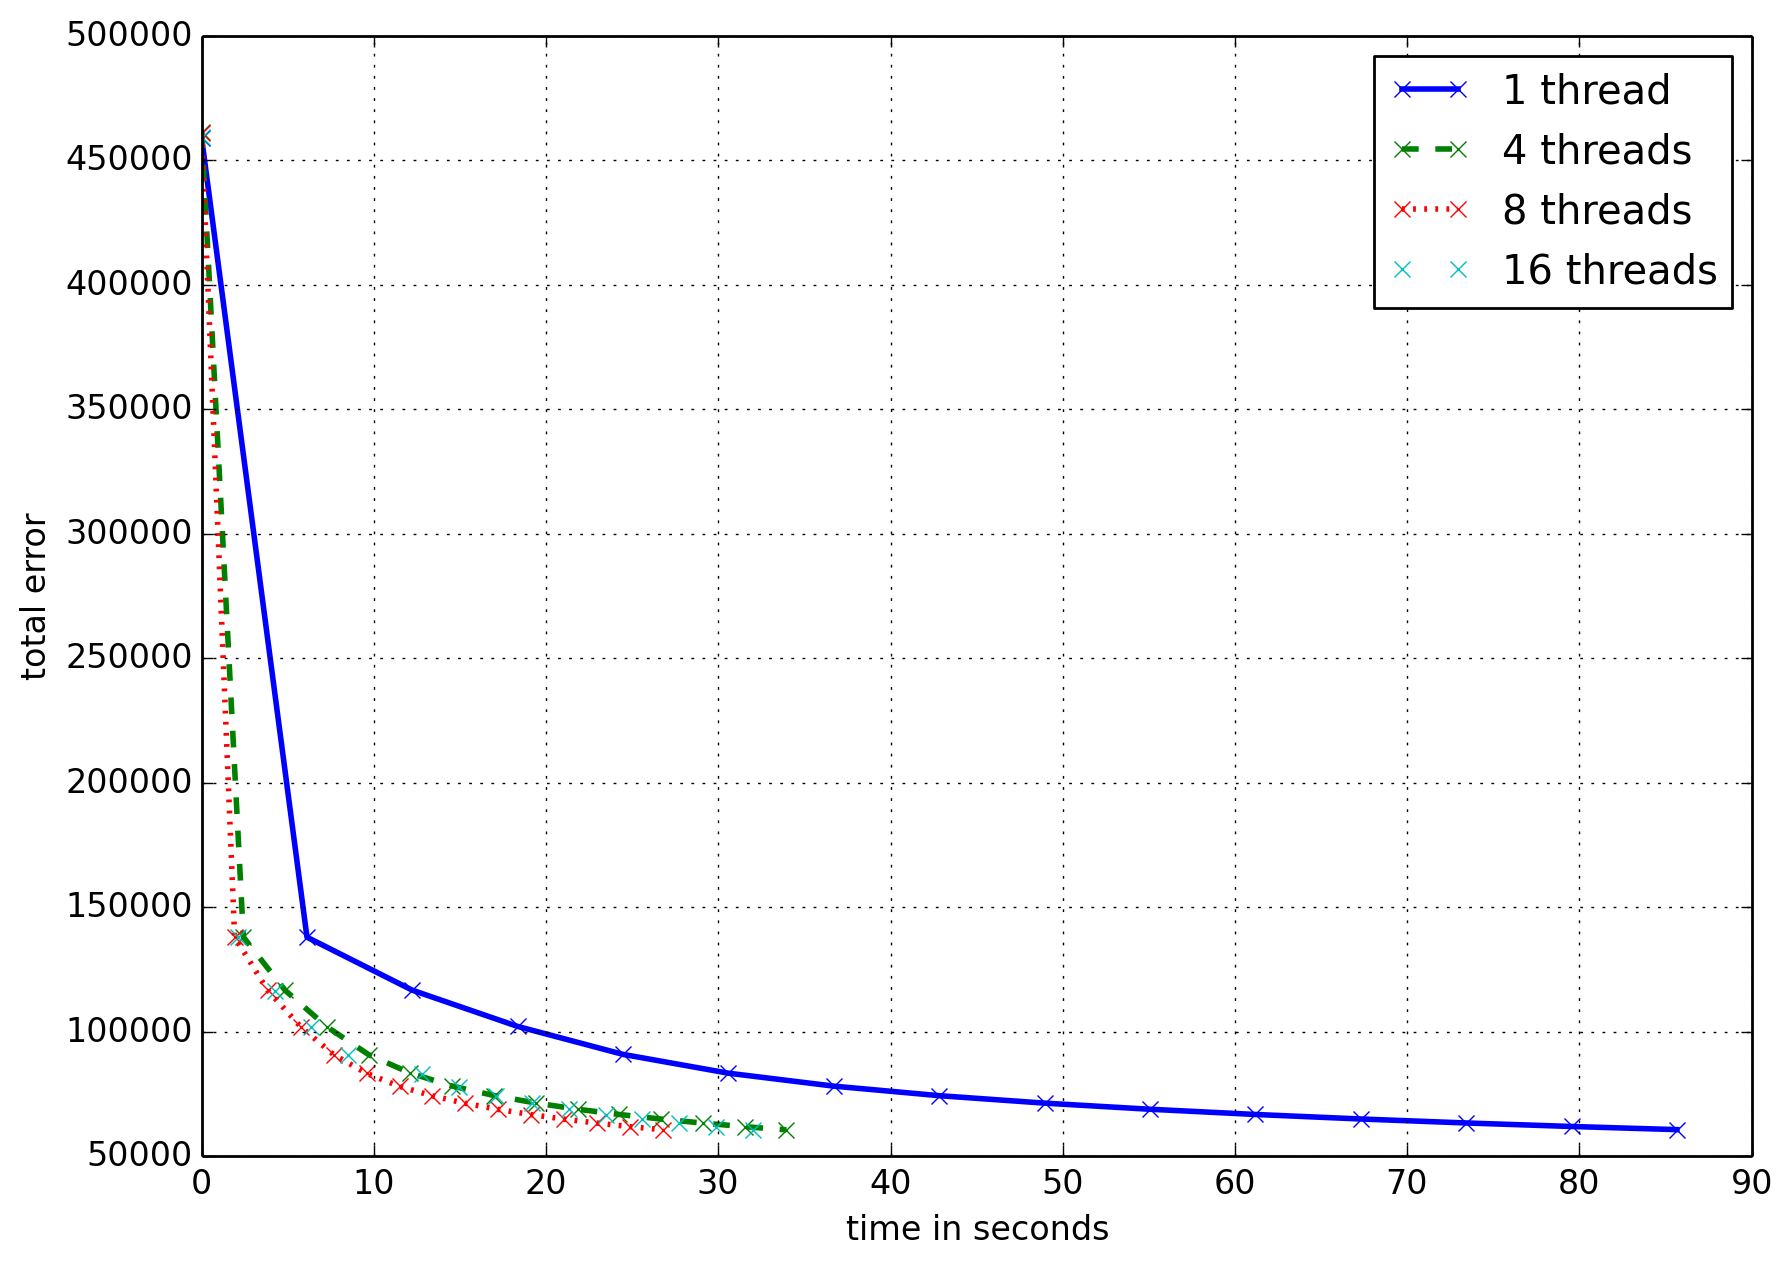
\includegraphics[width=0.8\linewidth]{experiment1SGD.png}
\caption{Performance results on a single autoencoder layer with 500 hidden nodes and trained for 15 iterations. Plot shows time elapsed versus total training error over 5000 images for 1, 4, 8, and 16 threads.}
\label{fig:experiment1}
\end{figure}


We note that the steps of backpropagation can only be done in sequence; thus we can only parallelize the operations done within each step. The three major operations which benefit from parallelization are computing the matrix-vector products $W^{H}x$ and $W^{O}y$, computing $\delta^O_j$ and $\delta^H_j$, and updating the entries of the weight matrices with the gradient. For performance reasons we don't store $W^O$ separately; instead we access $W^H$ with transposed indexes when decoding, calculating $\delta^O_j$, and applying the gradient update.

The most expensive parts of the backpropagation algorithm are computing the forward activations of the network and updating the weight matrices for the network. Computing the forward propagation requires performing a matrix-vector multiplication at each layer of the network. The size of that matrix depends on the input and output sizes of that layer. Thus if we have a network with $N$ layers and the sizes of each of those layers is $n_i$, then We have $N$ matrix-vector multiplications of size $n_{i-1} \times n_i$. Updating the weights also has complexity based on the size of the matrix since it requires updating all the entries of the matrix at each iteration.

To improve the performance of these two expensive steps, we parallelized them first using OpenMP and then later parallelized the matrix-vector products using OpenBLAS. Parallelization of these two steps is fairly straight forward and we give some results on scaling in Figs.~\ref{fig:performanceomp},~\ref{fig:performanceblas}, and \ref{fig:ompvsblas}.


\begin{figure}[h]
\centering
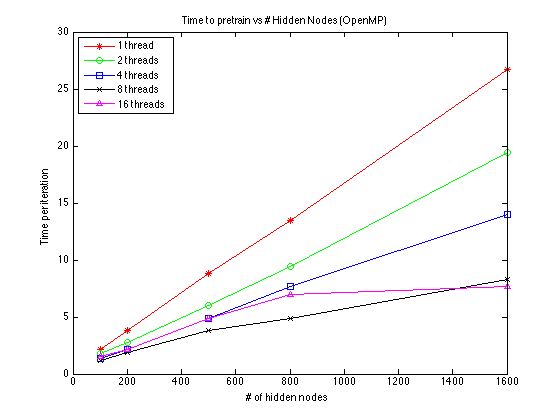
\includegraphics[width=0.8\linewidth]{performanceomp.png}
\caption{Time per iteration versus the number of threads and hidden nodes. We parallelize with our own OpenMP implementation and use 5000 training images.}
\label{fig:performanceomp}
\end{figure}


\begin{figure}[h]
\centering
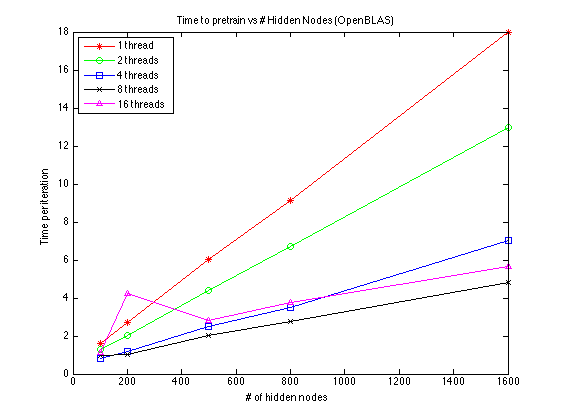
\includegraphics[width=0.8\linewidth]{performanceblas.png}
\caption{Time per iteration versus the number of threads and hidden nodes. We parallelize with OpenBLAS and we use 5000 training images.}
\label{fig:performanceblas}
\end{figure}

\begin{figure}[h]
\centering
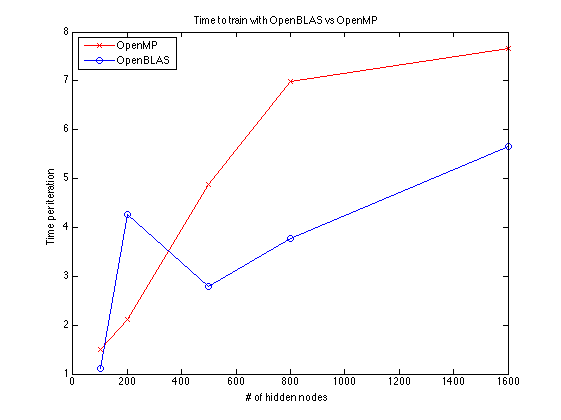
\includegraphics[width=0.8\linewidth]{ompvsblas.png}
\caption{Time per iteration versus parallelization technique and hidden nodes. We use 16 threads here.}
\label{fig:ompvsblas}
\end{figure}

In  Fig.~\ref{fig:performanceomp} we give the performance of training the autoencoder using SGD for different numbers of hidden nodes and different numbers of threads using our own parallel implementation.
In  Fig.~\ref{fig:performanceblas} we give the performance of training the autoencoder using SGD for different numbers of hidden nodes and different numbers of threads using OpenBLAS for parallelization of the matrix-vector multiplies and matrix-transpose-vector multiplies. The weight updates are not able to be done in OpenBLAS, and so we continue to do that using OpenMP. We consider the relative performance of these two methods in Fig.~\ref{fig:ompvsblas}.

We note that Figs.~\ref{fig:performanceomp} and~\ref{fig:performanceblas} show similar scaling, though in most cases the OpenBLAS version outperforms our own implementation. However, for small numbers of nodes, OpenBLAS does not perform well with many threads.
We generally get better perfomrance with a greater number of threads, but with a large number of threads we do not see improvement until the problem size increases and becomes large enough. We do not achieve linear scaling (i.e. twice as many threads does not result in the algorithm running twice as fast), since not all parts of the algorithm can be parallelized. 

\subsection{Visualization of Trained Weights and Reconstructed Images}

\begin{figure}[h] \centering
  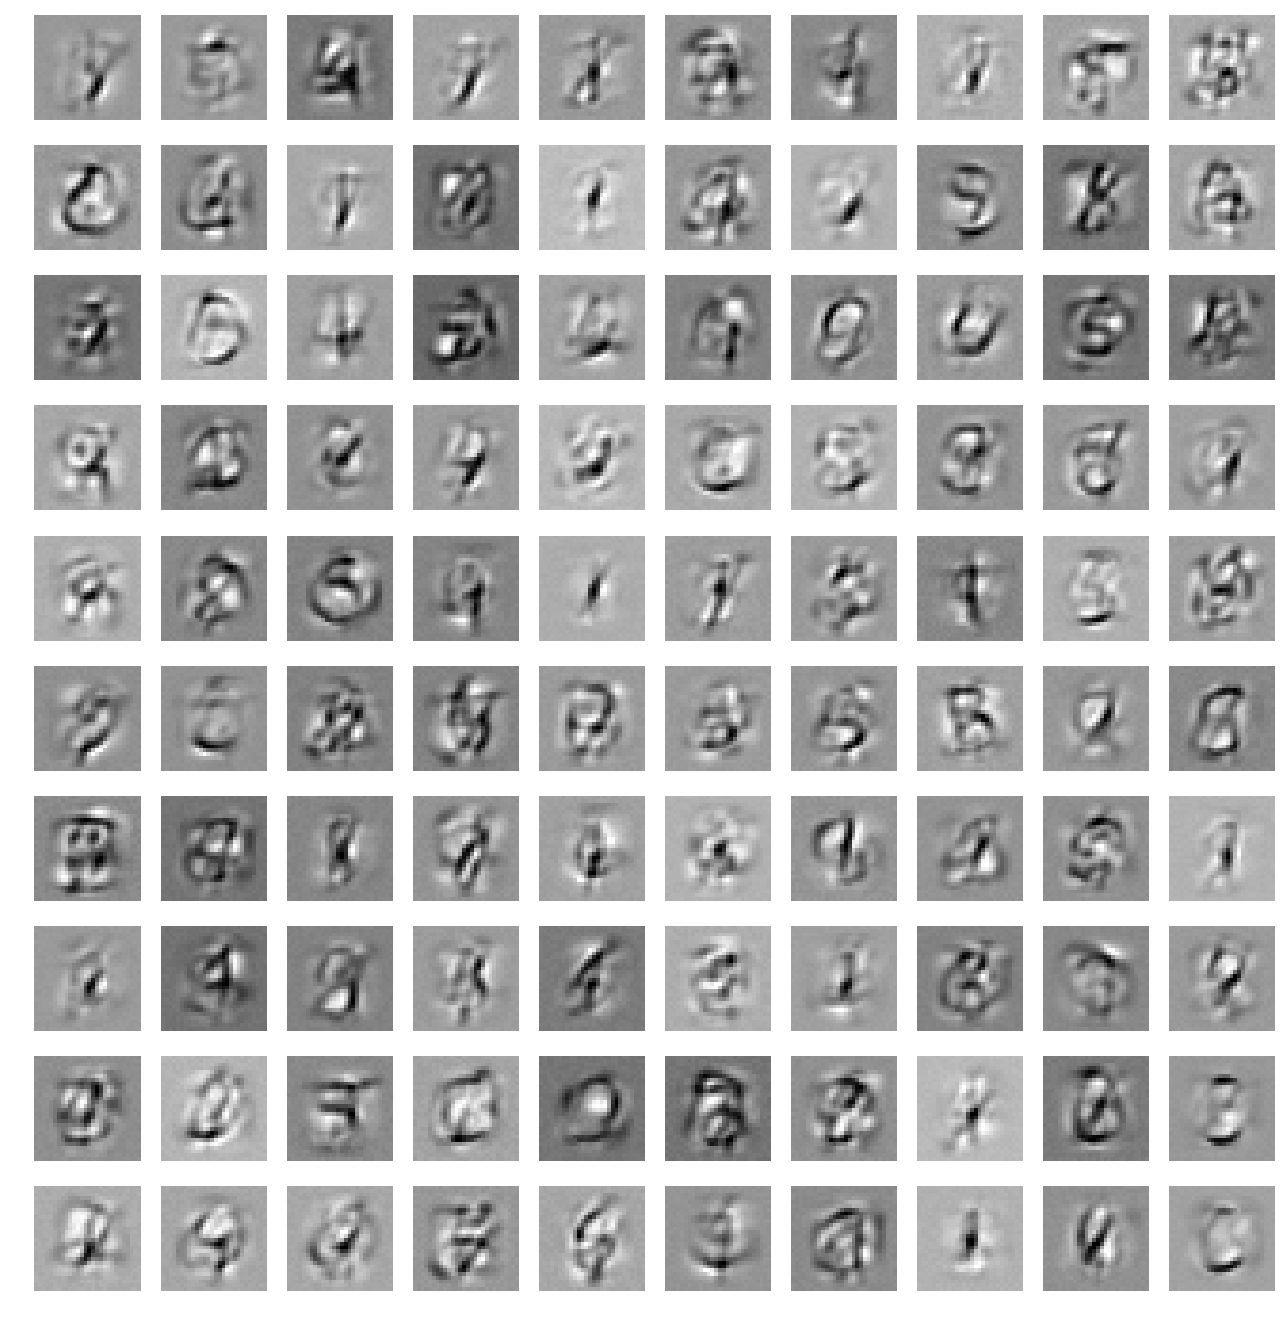
\includegraphics[width=0.8\linewidth]{experiment3_1.png}
  \caption{Visualization of the filters of the first 100 hidden nodes in an
  denoising autoencoder trained over all 60000 images.}
  \label{fig:experiment3_1}
\end{figure}

\begin{figure*}
  \centering
  \subfloat[]{
    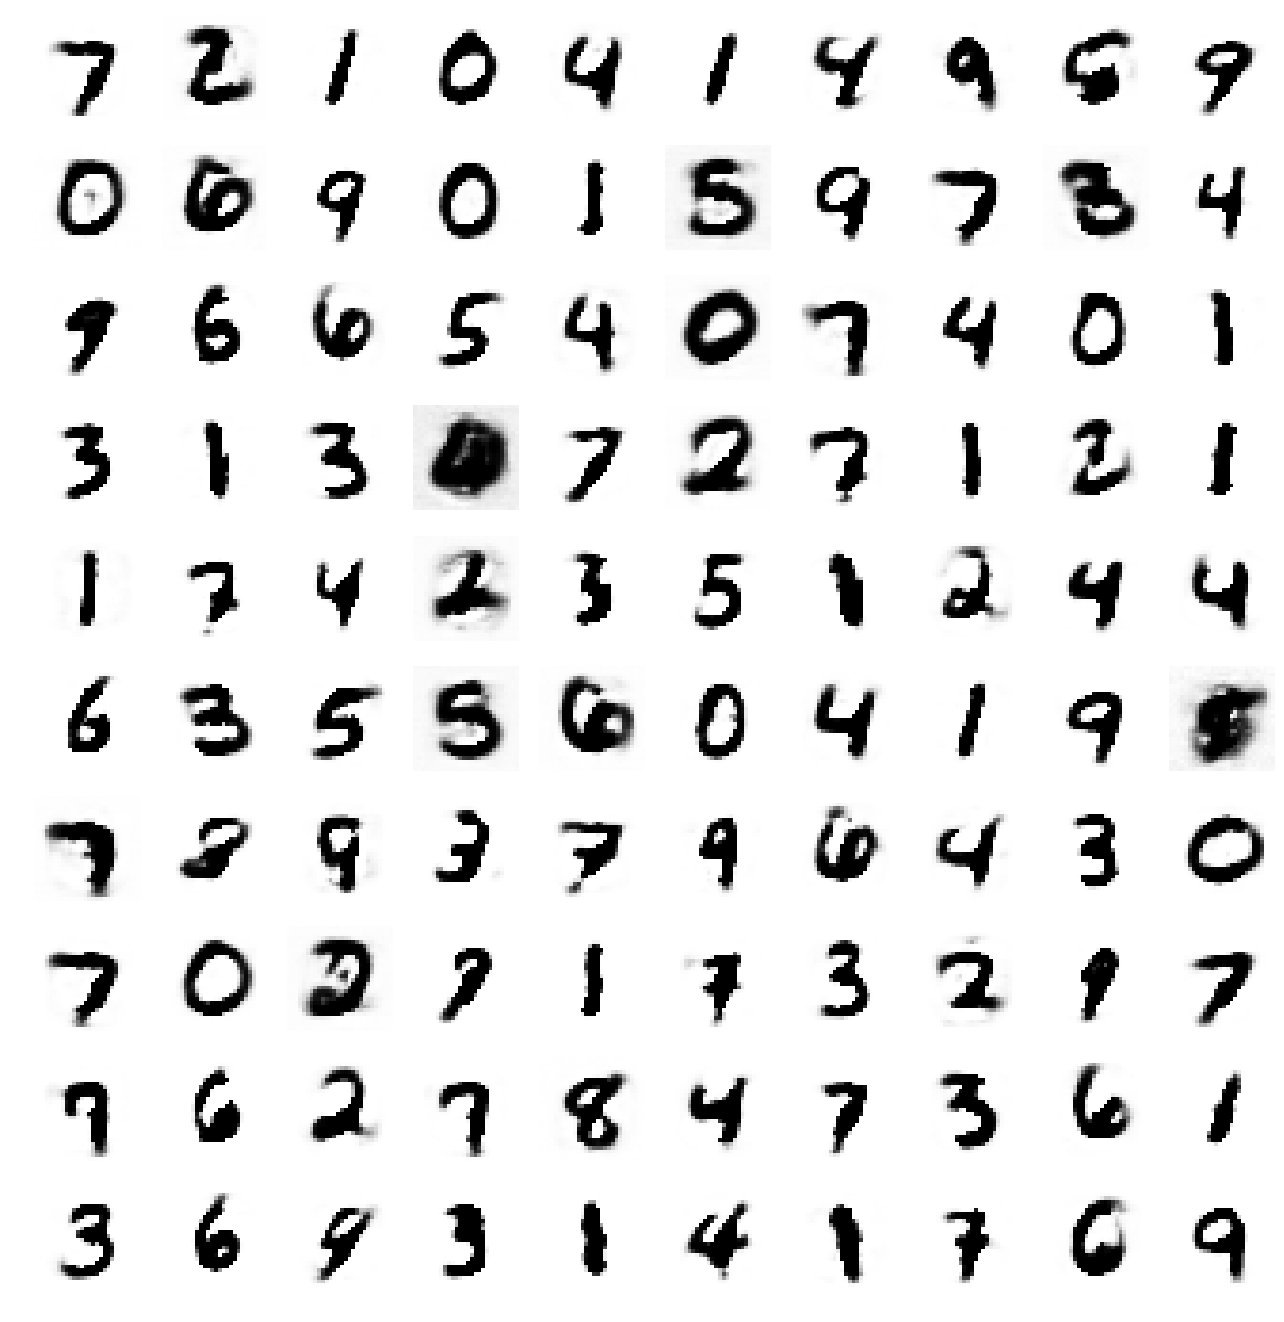
\includegraphics[width=0.4\linewidth]{experiment3_2.png}
  }
  \subfloat[]{
    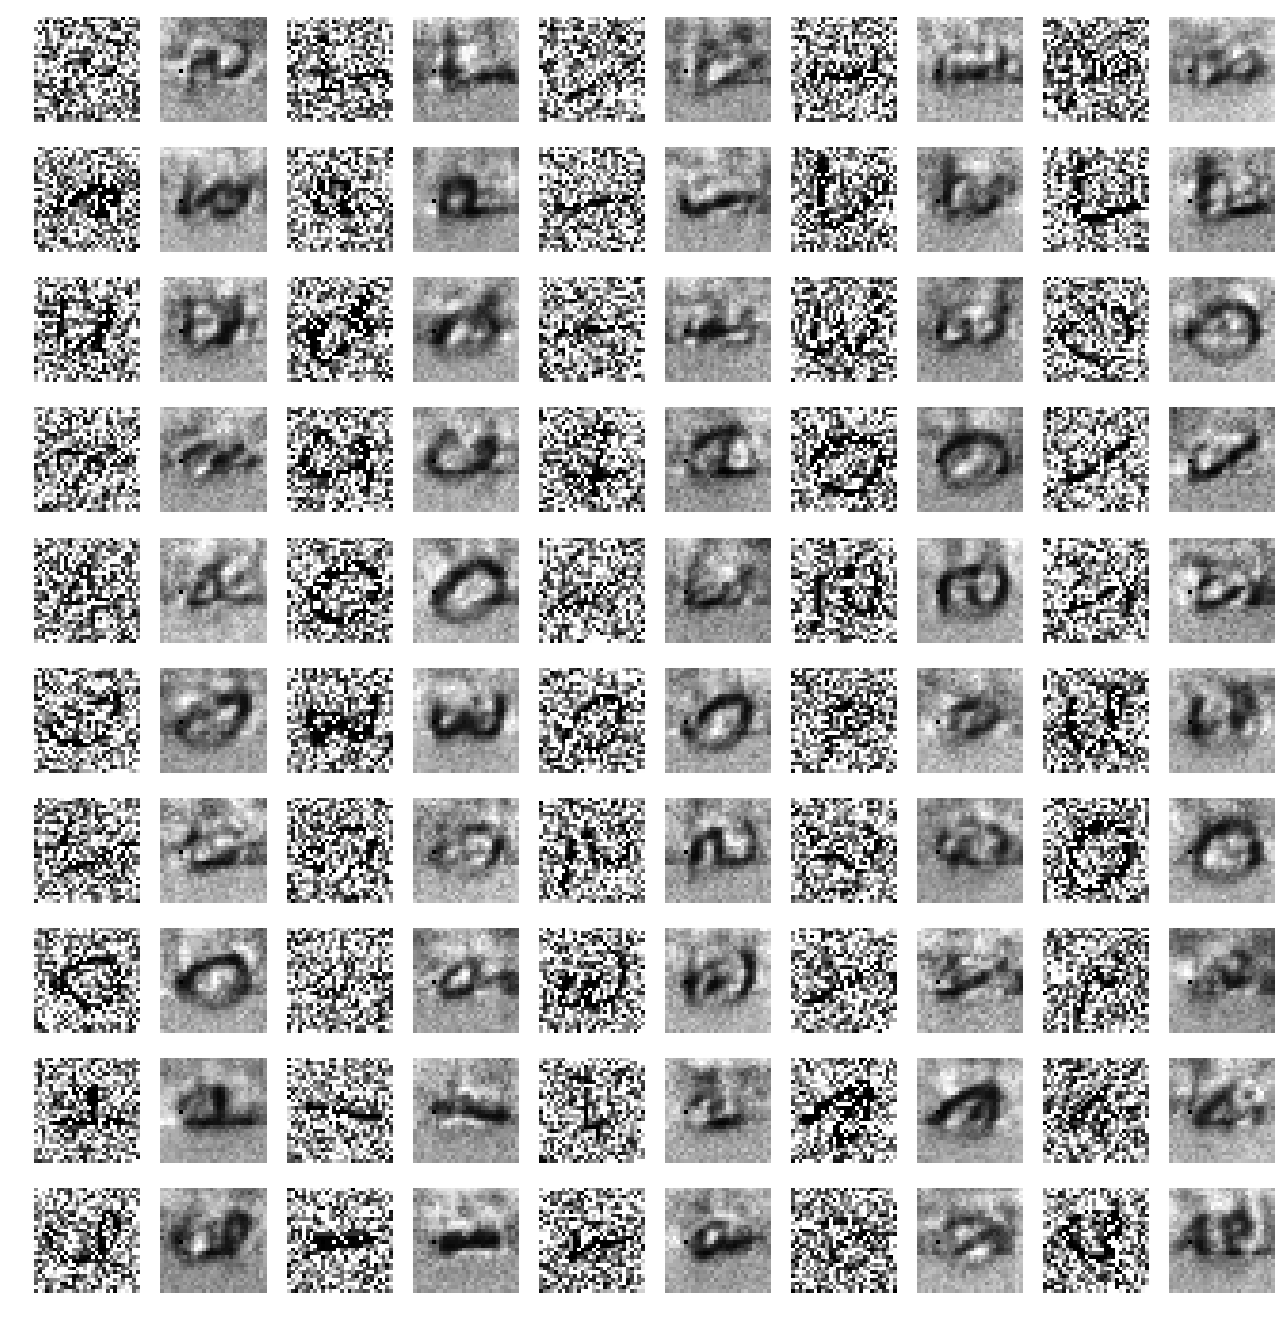
\includegraphics[width=0.4\linewidth]{rand.png}
  }
  \hspace{5mm}
  \subfloat[]{
    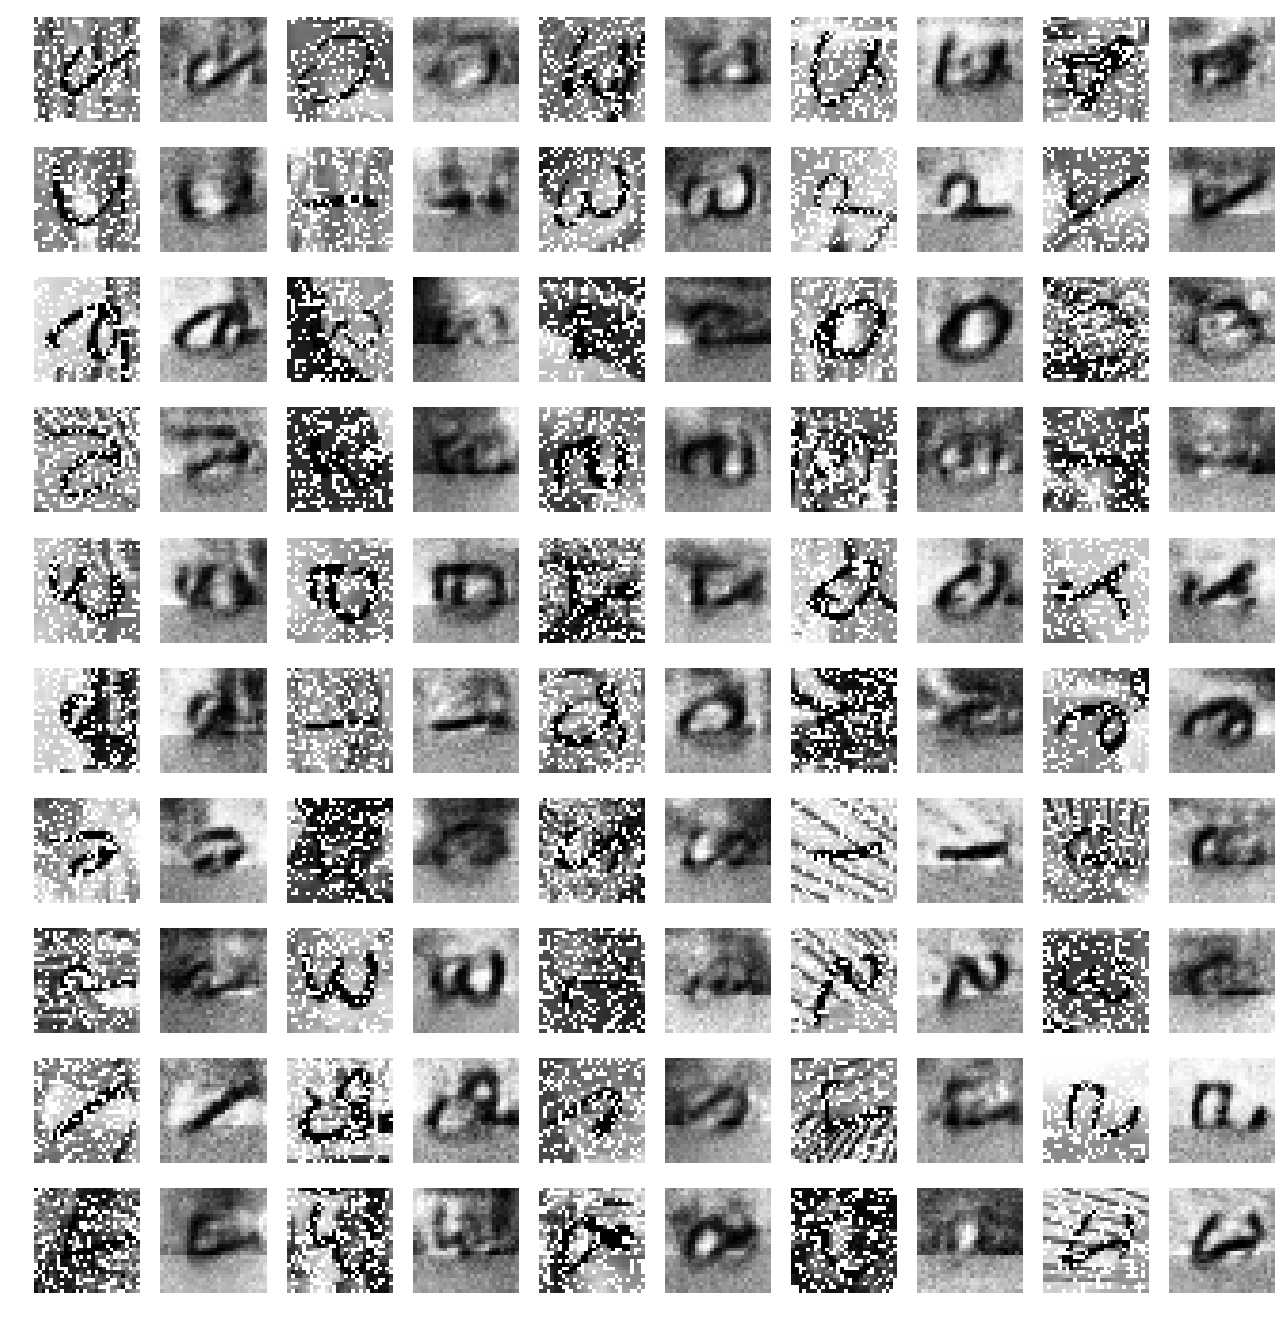
\includegraphics[width=0.4\linewidth]{bg.png}
  }
  \subfloat[]{
    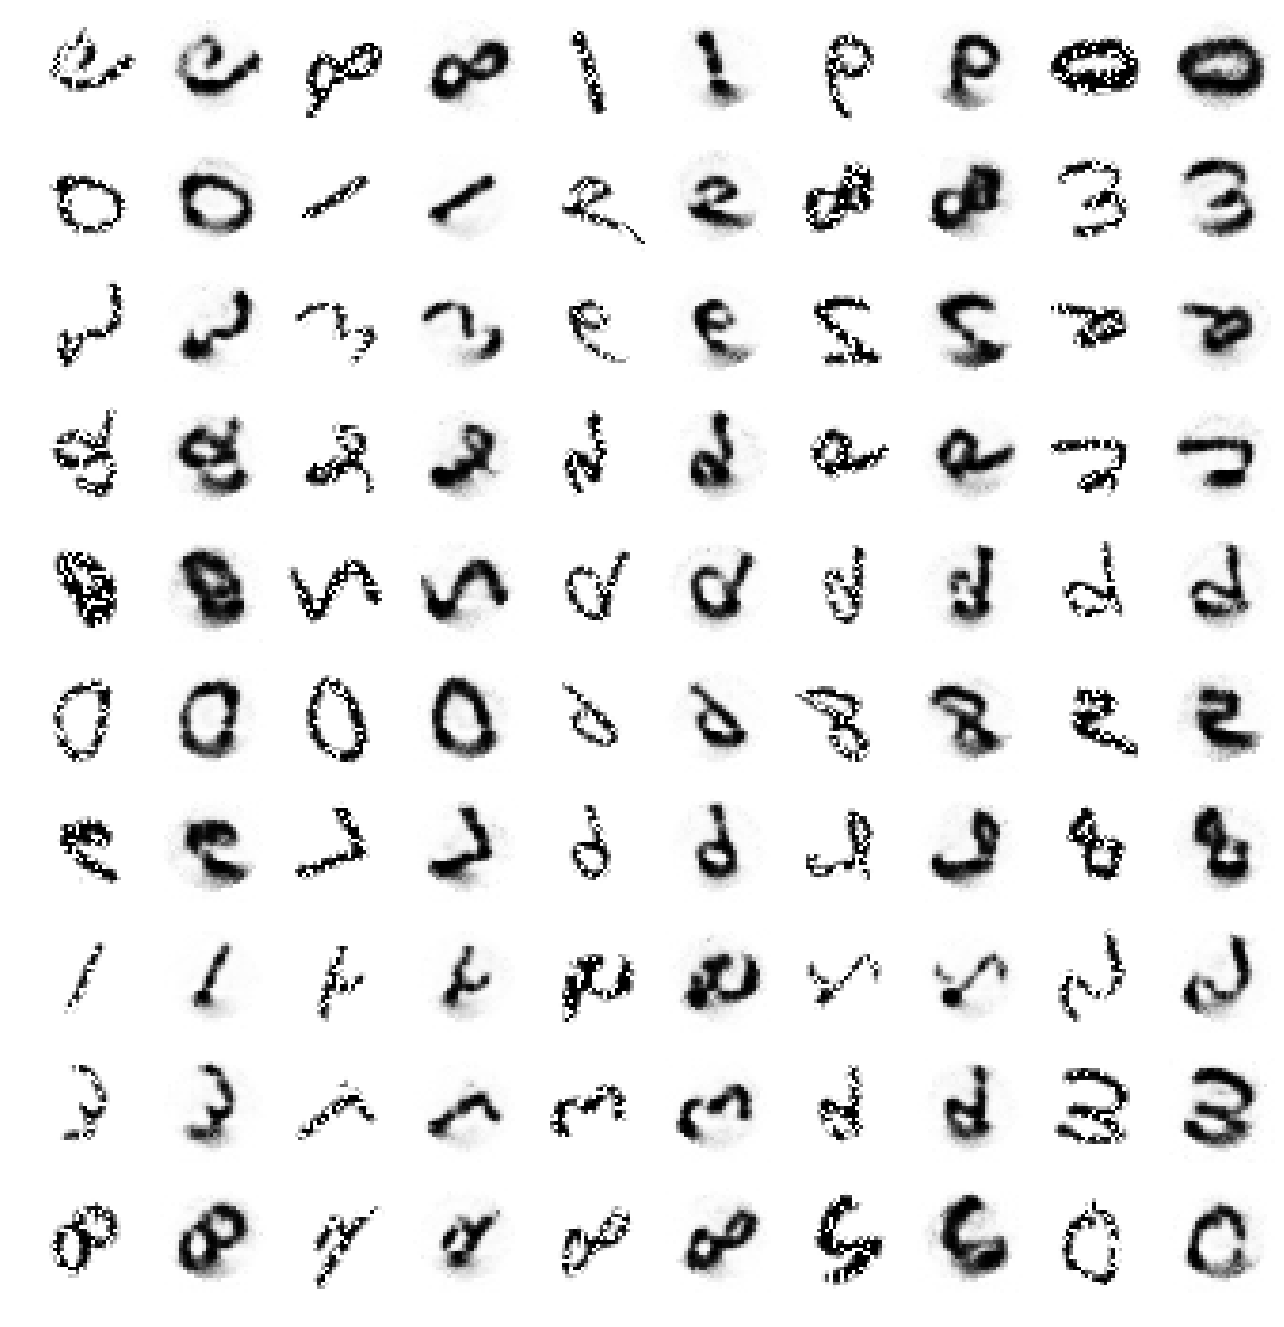
\includegraphics[width=0.4\linewidth]{rot.png}
  }
  \caption{Reconstructions of corrupted digits from the (a) MNIST dataset (b) bg-rand dataset, (c) bg-img dataset, and (d) rot dataset}
  \label{fig:reconstruct}
\end{figure*}

Next, in Fig.~\ref{fig:experiment3_1}, we visualize the filters that are
learned by training an autoencoder layer with 500 hidden nodes over all 60000
training images. The  filter for each hidden node is a row vector of the weight
matrix and indicates which aspects of the input the hidden unit is sensitive
to. Since each row in the weight matrix is the same dimensionality as the
input, we can visualize it as a 28 by 28 pixel image. The filters are not
identical to the input images, but do show some similarity to them. In
Fig.~\ref{fig:reconstruct}, we visualize the reconstructed digits when given
noisy test digits as input. The reconstructed outputs for most of the input
images are easily recognizable as digits, which indicates that the autoencoder
is indeed denoising and learning a good representation of the images.

To further demonstrate the reconstruction capabilities of the autoencoder, we
trained the autoencoder on corrupted or otherwise altered digits.  In
particular, we test the reconstruction on \textit{bg-rand}, which is generated
from the MNIST dataset, except that a random background is added. In
\textit{bg-img}, each image is given a background randomly selected from one of
twenty images downloaded from the internet. In \textit{rot}, the digits are
simply rotated by some random angle.  These alterations to the images make the
classification task more difficult. Indeed the digits are very difficult to
identify, but the autoencoder creates an easier to identify representation,
even to the human eye. We show also in Fig.~\ref{fig:reconstruct} the
reconstructed images form the \textit{bg-img} and \textit{rot} datasets. Note
that the images in the \textit{bg-rand} and \textit{bg-img} datasets are
rotated, but they are all rotated in the same way.

Finally we evaluate the classification accuracy of a deep neural network that
has multiple stacked denoising autoencoders. We train 3 stacked autoencoder
layers, each with 1000 hidden units, and using noise levels 0.1, 0.2, and 0.3
respectively. Each layer is trained for 15 iterations with a learning rate of
0.001. After the unsupervised pretraining, a conventional feed-forward network
with 1000 input units, 500 hidden units and 10 outputs is connected to the
hidden units of the last autoencoder layer. This conventional network is then
trained for 30 iterations (learning rate 0.1) in a supervised manner, where the
target $t$ is the indicator vector representation of the training label. Our
final classification accuracy is 98.04\%. In comparison, the best reported accuracy achieved
with a SVM with RBF kernel is 98.60\% \cite{vincent2010stacked}.

\subsection{Representation Learning for Supervised Classification}

Recall that one of the main reasons for using an autoencoder is to determine a
more useful representation of the data for other tasks, for example in a
classification task. To this end, we constructed and trained (15 iterations) an
autoencoder with just a single layer and 1000 hidden units and used it to
create a more useful representation of the digits in the MNIST dataset. After
this more useful representation is constructed, we can then use the output from
the autoencoder as input to another type of classification algorithm.  Since
the autoencoder produces a better representation of the data, we expect that
given the encoded data, the other classification algorithms should perform
better.  The results of these experiments is given in
Table.~\ref{tab:classvsenc}.

To test this, we used liblinear \cite{fan2008liblinear} to attempt to train a model and then predict on
a test set for both the original and encoded datasets. With the original data
liblinear gives an accuracy of 91.68\% on the test set when using the default
parameters. However, when the encoded data from the trained autoencoder gives
an accuracy of 97.07\%. This is a nontrivial improvement in the classification
accuracy. Thus, the autoencoder has created a better representation of the data
which made it easier for liblinear to classify. This verifies that the
autoencoder is doing what it is expected to do.

Similarly, we performed the same experiment as above, except in this case we
used libsvm with an RBF kernel and all the default parameters.  Without
encoding the data first, we get an accuracy of 94.46\%, but using the encoded
data gives a prediction accuracy of 95.48\%. As above, the encoded data allows libsvm
better classify the data. We should note that our accuracy is not as good as the one reported earlier as we did not tune the hyperparameters (C and kernel width) of the SVM classifier. 

Using logistic regression to perform the classification, we experienced similar results.
Again we use liblinear with all default options except selecting logistic regression. Using the
original MNIST data, this algorithm achieved an accuracy of 91.82\% while with the encoded data
we achieved an accuracy of 96.86\%.

We performed the same experiments on the \textit{bg-rand}, \textit{bg-img} and 
\textit{rot} datasets as well. Across the board we see similar results. The encoding does not have much of
an effect on the ability of kernel SVM to classify the data, but for linear SVM and logistic regresssion, 
using the autoencoder always results in the classifier improving it's accuracy. 


\begin{table}[h]
	\centering
\begin{tabular}{ll|lll}
    Dataset                        & Data               & Linear SVM & Kernel SVM (RBF) & Logistic Regression \\ \hline
    \multirow{2}{*}{MNIST}         & Original           & 91.68\%    & 94.46\%          & 91.82\%             \\
                                   & Encoded            & 97.07\%    & 95.48\%          & 96.86\%             \\ \hline
    \multirow{2}{*}{mnist-bg-rand} & Original           & 58.975\%   & 83.875\%         & 65.5917\%           \\
                                   & Encoded            & 81.675\%   & 83.6583\%        & 83.825\%            \\ \hline
    \multirow{2}{*}{mnist-bg-img}  & Original           & 69.25\%    & 76.4667\%        & 71.6333\%           \\
                                   & Encoded            & 78.4333\%  & 72.8417\%        & 78.1333\%           \\ \hline
    \multirow{2}{*}{mnist-rot}     & Original           & 11.204\%   & 13.328\%         & 11.868\%           \\
                                   & Encoded            & 18.428\%   & 14.378\%         & 18.78\%
\end{tabular}
	\caption{Summary of the results of running different classification algorithms on the raw MNIST data and on the output from a trained autoencoder. We
	see in all cases that using the encoded data produces a better result.}
	\label{tab:classvsenc}
\end{table}

\subsection{Genetic Algorithms}

\begin{table}[h]
  \centering
\begin{tabular}{l|l}
Hyperparameter     & Value                                                          \\ \hline
Mutation Rate $mr$ & $0.0001$ \\
Mutation Amount $ma$ & $0.1r$ \\
Crossover Rate $mr$ & $0.5$ \\
Population Size $N$ & $2$ \\
Replacement Fraction $\alpha$ & $0.5$ \\
Initial Value Range $r$ & $1/\sqrt{\text{FANIN}}$ \\
Power Scaling Parameter $\gamma$ & $1.0$ \\
Backpropagation Fraction $\beta$ (HGA only) & $0.5$ \\ 

\end{tabular}
\caption{List of hyperparameters for CGA and HGA. FANIN is input dimensionality of autoencoder layer.}
\label{tab:hyperparameters}
\end{table}

\begin{figure}[h] \centering
  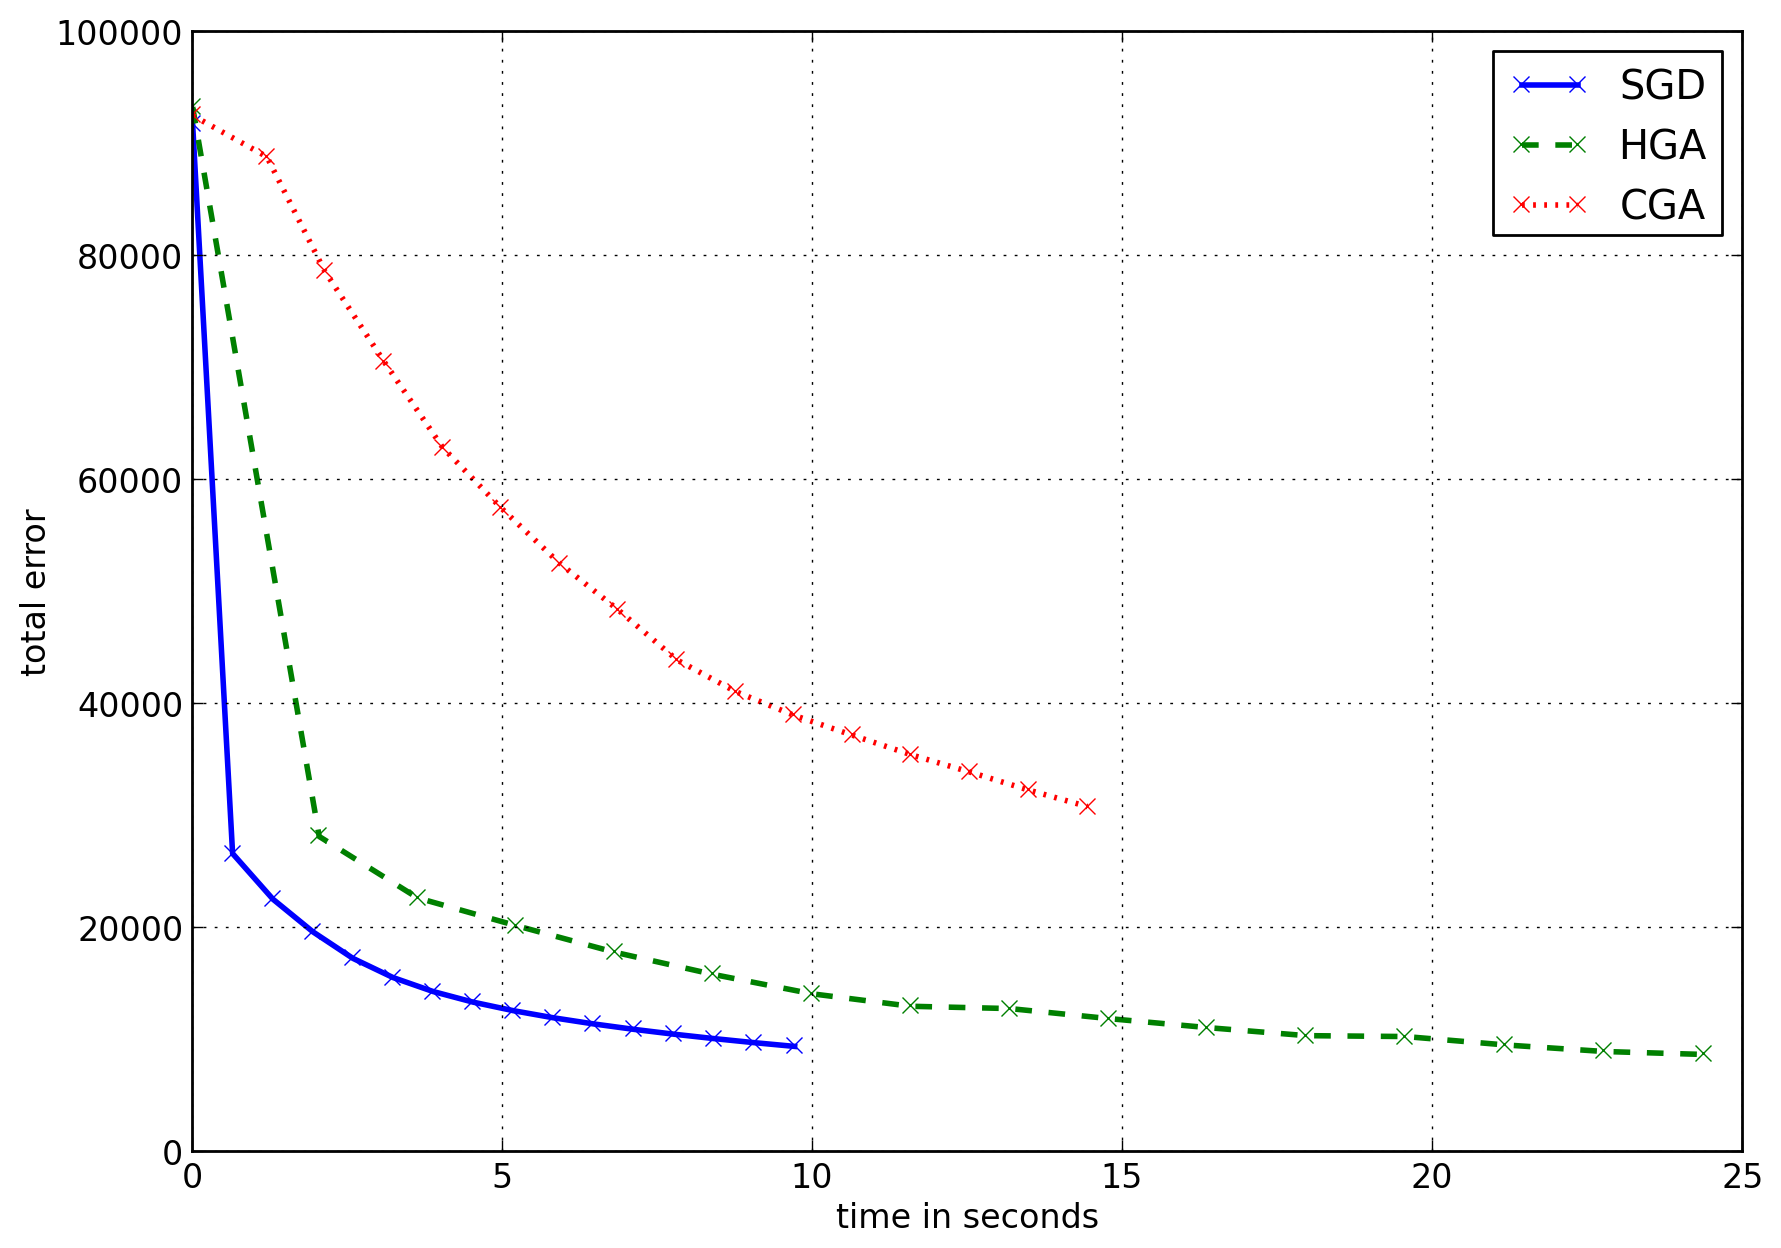
\includegraphics[width=0.8\linewidth]{ga_comparison.png}
  \caption{Comparison of the performance of SGD, HGA, and CGA. SGD is fastest, while HGA achieves the lowest reconstruction error. HGA and CGA uses a default population size of 2 and all three algorithms cycle through 1000 training images for 15 iterations.}
  \label{fig:ga_comparison}
\end{figure}

For all of the following experiments, we train a single autoencoder layer with 1000 hidden units and cycle through 1000 training digits for 15 iterations. The default hyperparameters for CGA and HGA are listed in Table.~\ref{tab:hyperparameters}. To parallelize the GA, we modified the mutation and crossover operators to support multiple threads. Because mutation and crossover modifies each element of the individual independently, no locking is required. The computation of an individual's fitness is already parallelized since it reuses the same code from SGD for determining the least squares loss. The remaining operations of the GA does not need parallelization since they are computationally cheap. 

In Fig.~\ref{fig:ga_comparison}, we compare the performance of SGD, HGA (uses backpropagation to update the best individuals in the population), and CGA (does not use any gradient information). SGD is the fastest by roughly a factor of two when compared to HGA, while CGA is somewhere in between. However, HGA is able to achieve the lowest reconstruction error (8709 vs SGD's 9427). CGA performed the worst out of all three algorithms, having a reconstruction error that is three times larger than that of the other algorithms. The hyperparameters for HGA and CGA are hand tuned and not necessary optimal. However, we believe that with properly tuned hyperparameters, HGA might be competitive with SGD for both final reconstruction error and performance time. 

Next in Fig.~\ref{fig:ga_comparison2}, we examine the scalability of HGA. HGA shows roughly 3x speedup when using 4 threads, 5x speedup when using 8 threads, and 6x speedup when using 16 threads. The performance improvement versus the number of threads is sublinear and can be attributed to two main causes: 1) Cache conflicts when performing mutation and crossover due to multiple threads writing and reading different memory locations, 2) The sequential nature of backpropagation, which HGA utilizes to help optimize the weights. However, HGA does seem to have moderately better scalability than our parallel implementation of SGD. This is attributable to the fact that the mutation and crossover operators are very straightforward to parallelize and scale in performance very well. 

In Fig.~\ref{fig:ga_comparison3}, the performance of HGA versus the number of threads and number of hidden units in autoencoder layers is visualized for both a population size of 50 and the default size of 2. As we can see, the HGA's performance scales linearly with the number of hidden units and that this relationship holds even when the population size is increased to 50. Interestingly, the performance when using 8 or 16 threads is not distinguishable for small numbers of hidden units. This is probably due to the computational overhead that result from creating additional threads.

Finally, in Fig.~\ref{fig:ga_comparison4}, we plot the performance of CGA and HGA for population sizes of 2, 4, 8, 16, and 32. All other hyperparameters remain the same for both HGA and CGA. As we can see, larger populations does lead to a noticeable improvement in the final reconstruction error, but at a cost of increased running time that is linear in the population size. For each fixed population size, HGA performs significantly better than CGA, with a final construction error is roughly 10 times lower. However for a given population size, HGA does take 40\% to 50\% longer to finish; this is attributable to the fact that CGA does not perform backpropagation, which takes additional time. 

\begin{figure}[h] \centering
  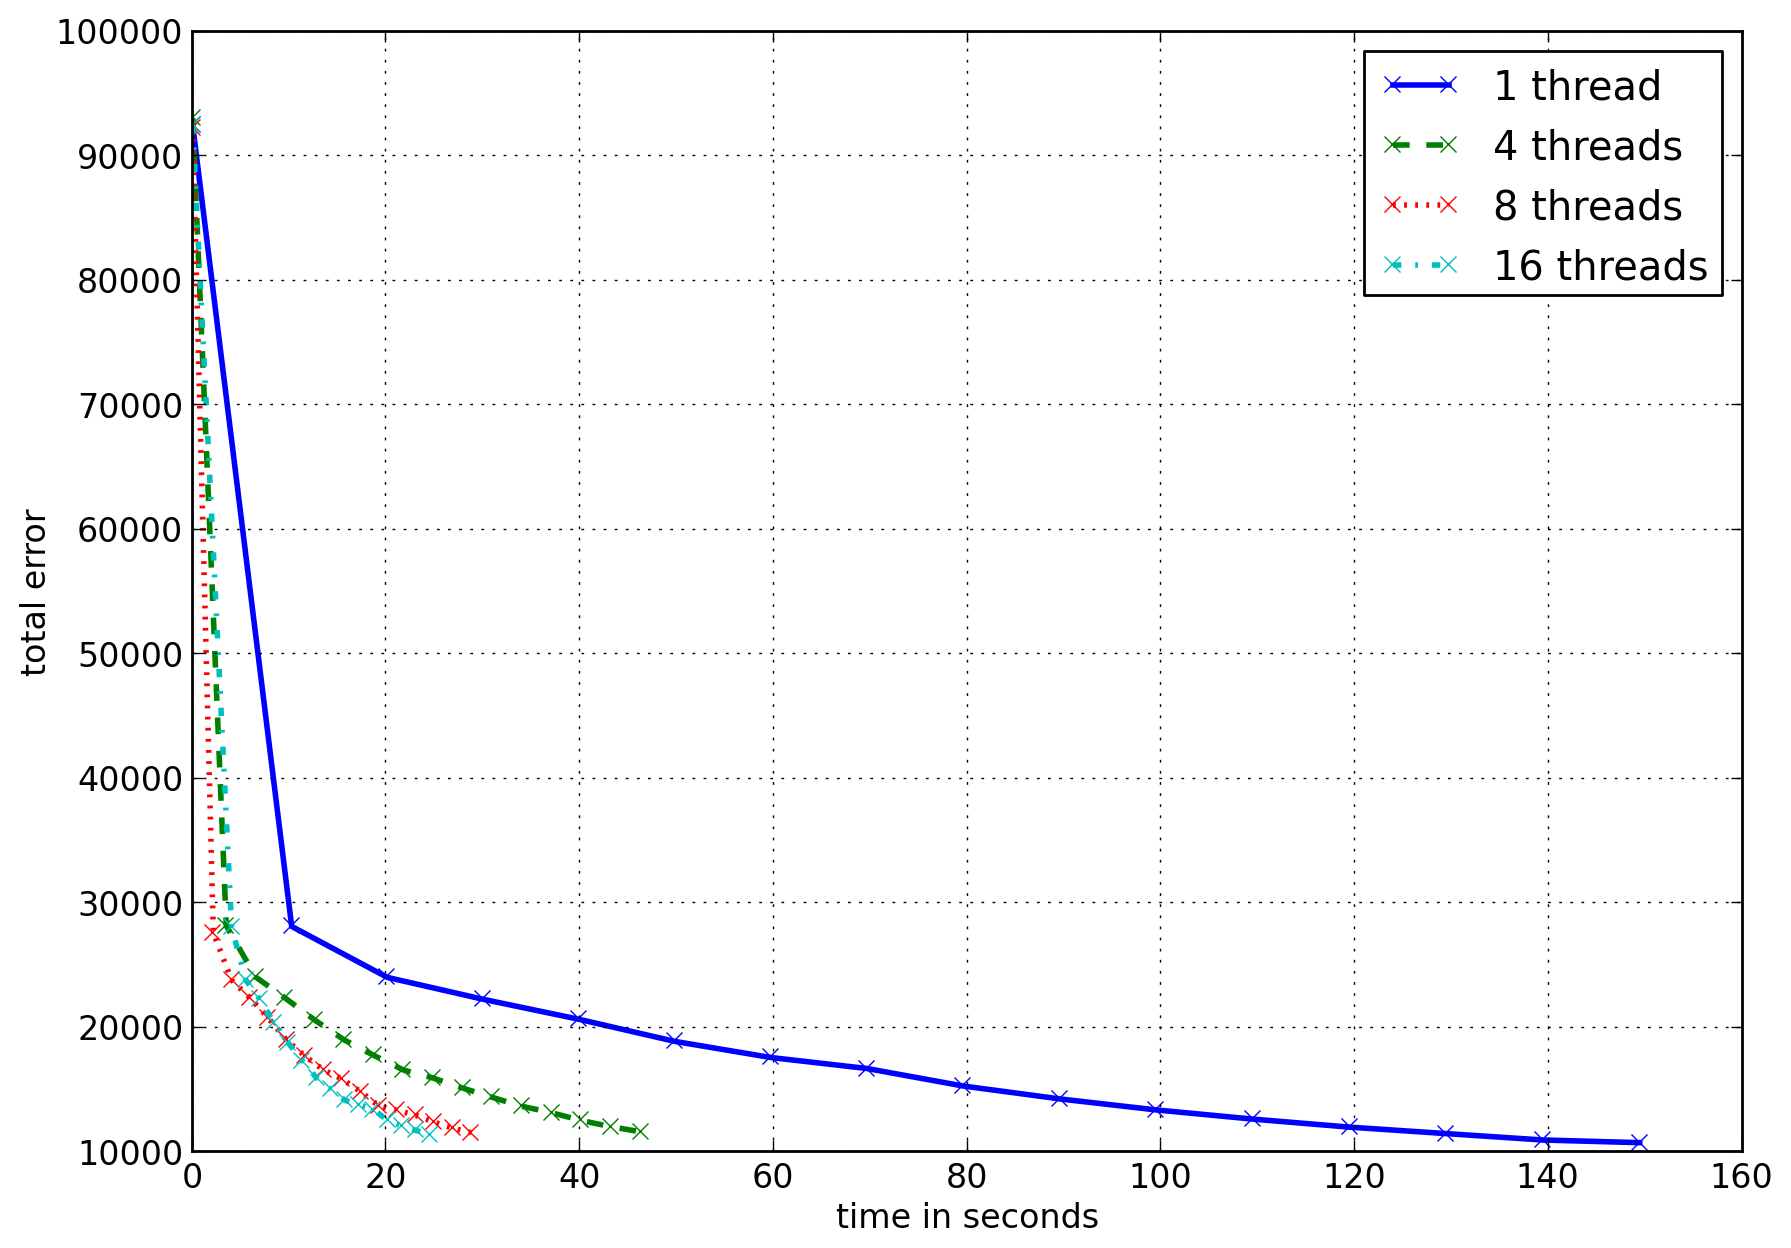
\includegraphics[width=0.8\linewidth]{ga_comparison2.png}
  \caption{Performance of HGA for 1, 4, 8, and 16 threads with a population size of 2 and 1000 training images.}
  \label{fig:ga_comparison2}
\end{figure}

\begin{figure*}[h]
  \centering
  \subfloat[]{
    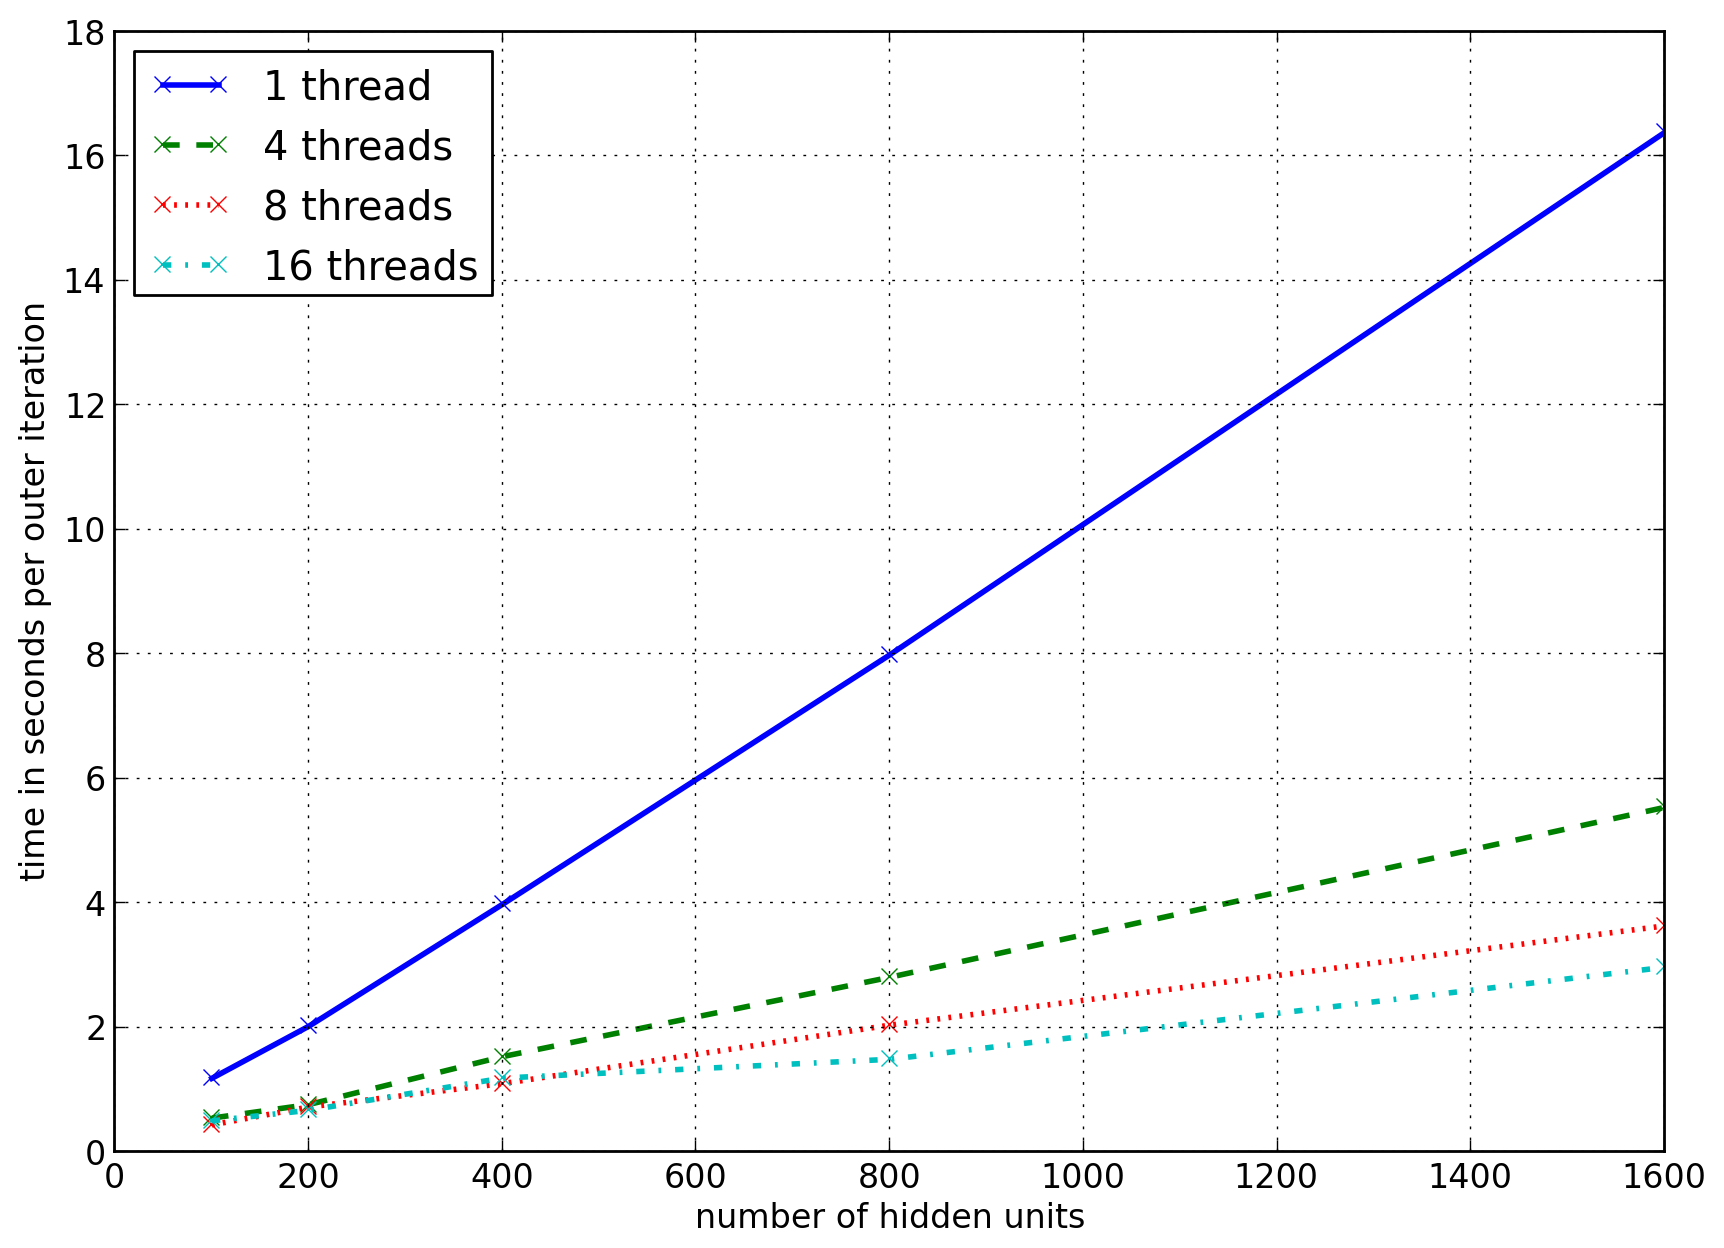
\includegraphics[width=0.45\linewidth]{ga_comparison3.png}
  }
  \subfloat[]{
    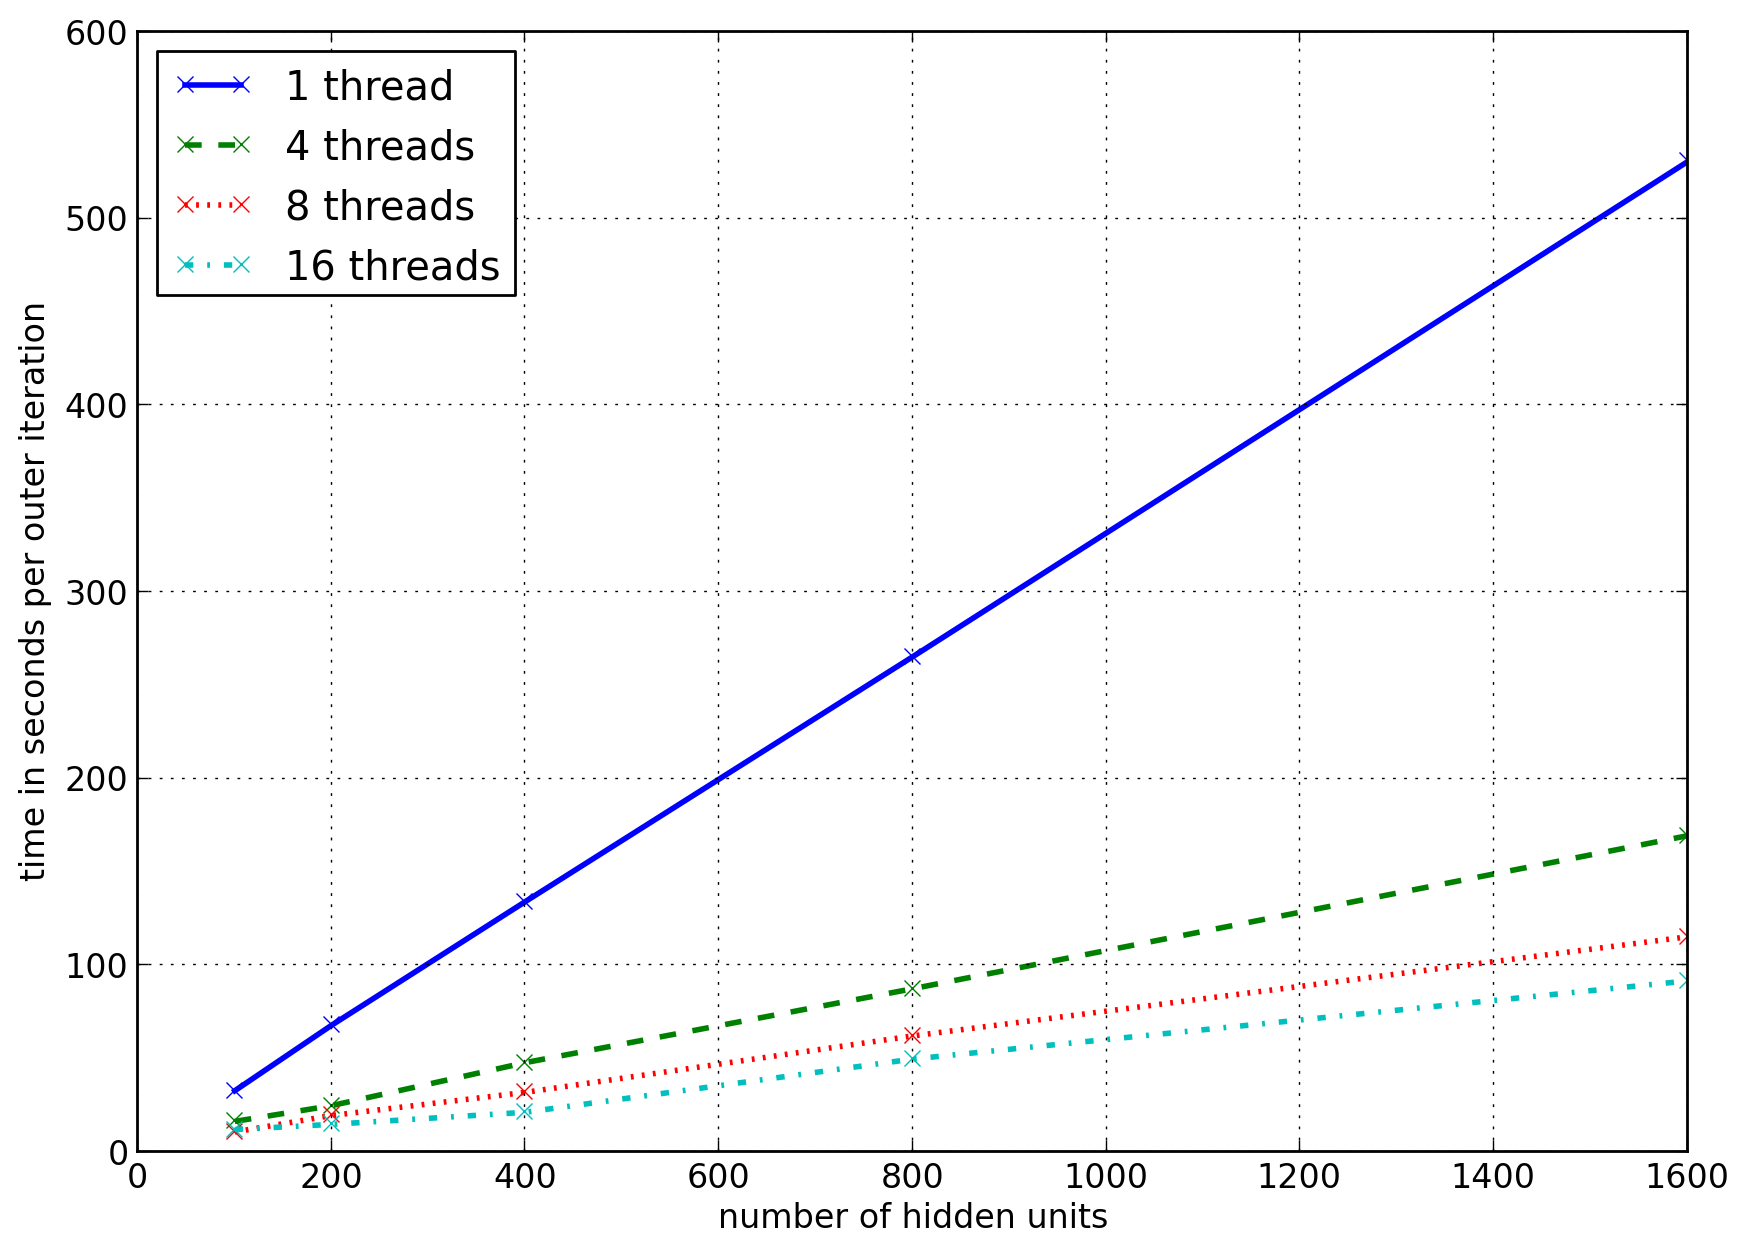
\includegraphics[width=0.45\linewidth]{ga_comparison3_big.png}
  }
  \caption{Comparison of performance versus number of threads and number of hidden units in autoencoder layer for HGA with population size (a) 2 and (b) 50.}
  \label{fig:ga_comparison3}
\end{figure*}

\begin{figure*}[h]
  \centering
  \subfloat[]{
    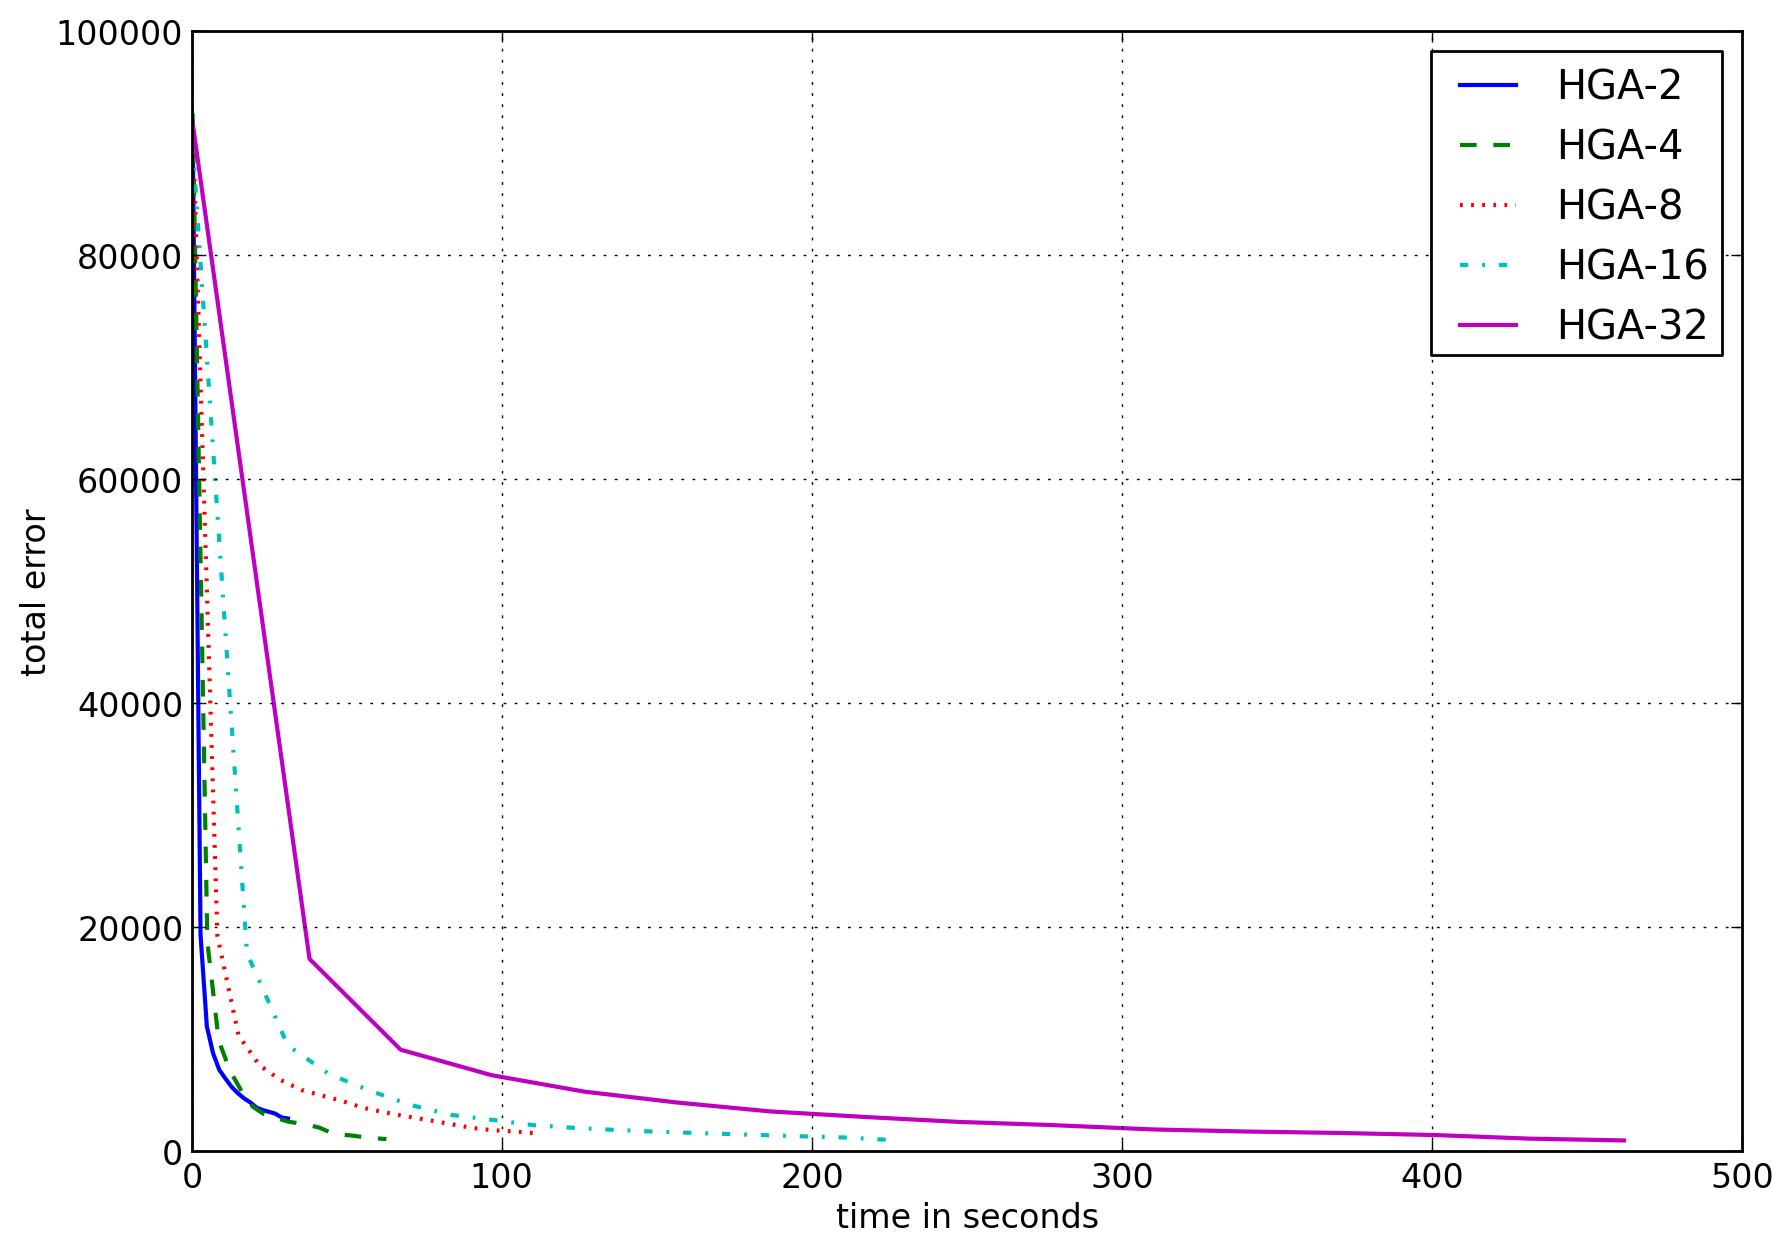
\includegraphics[width=0.45\linewidth]{ga_comparison4_1.png}
  }
  \subfloat[]{
    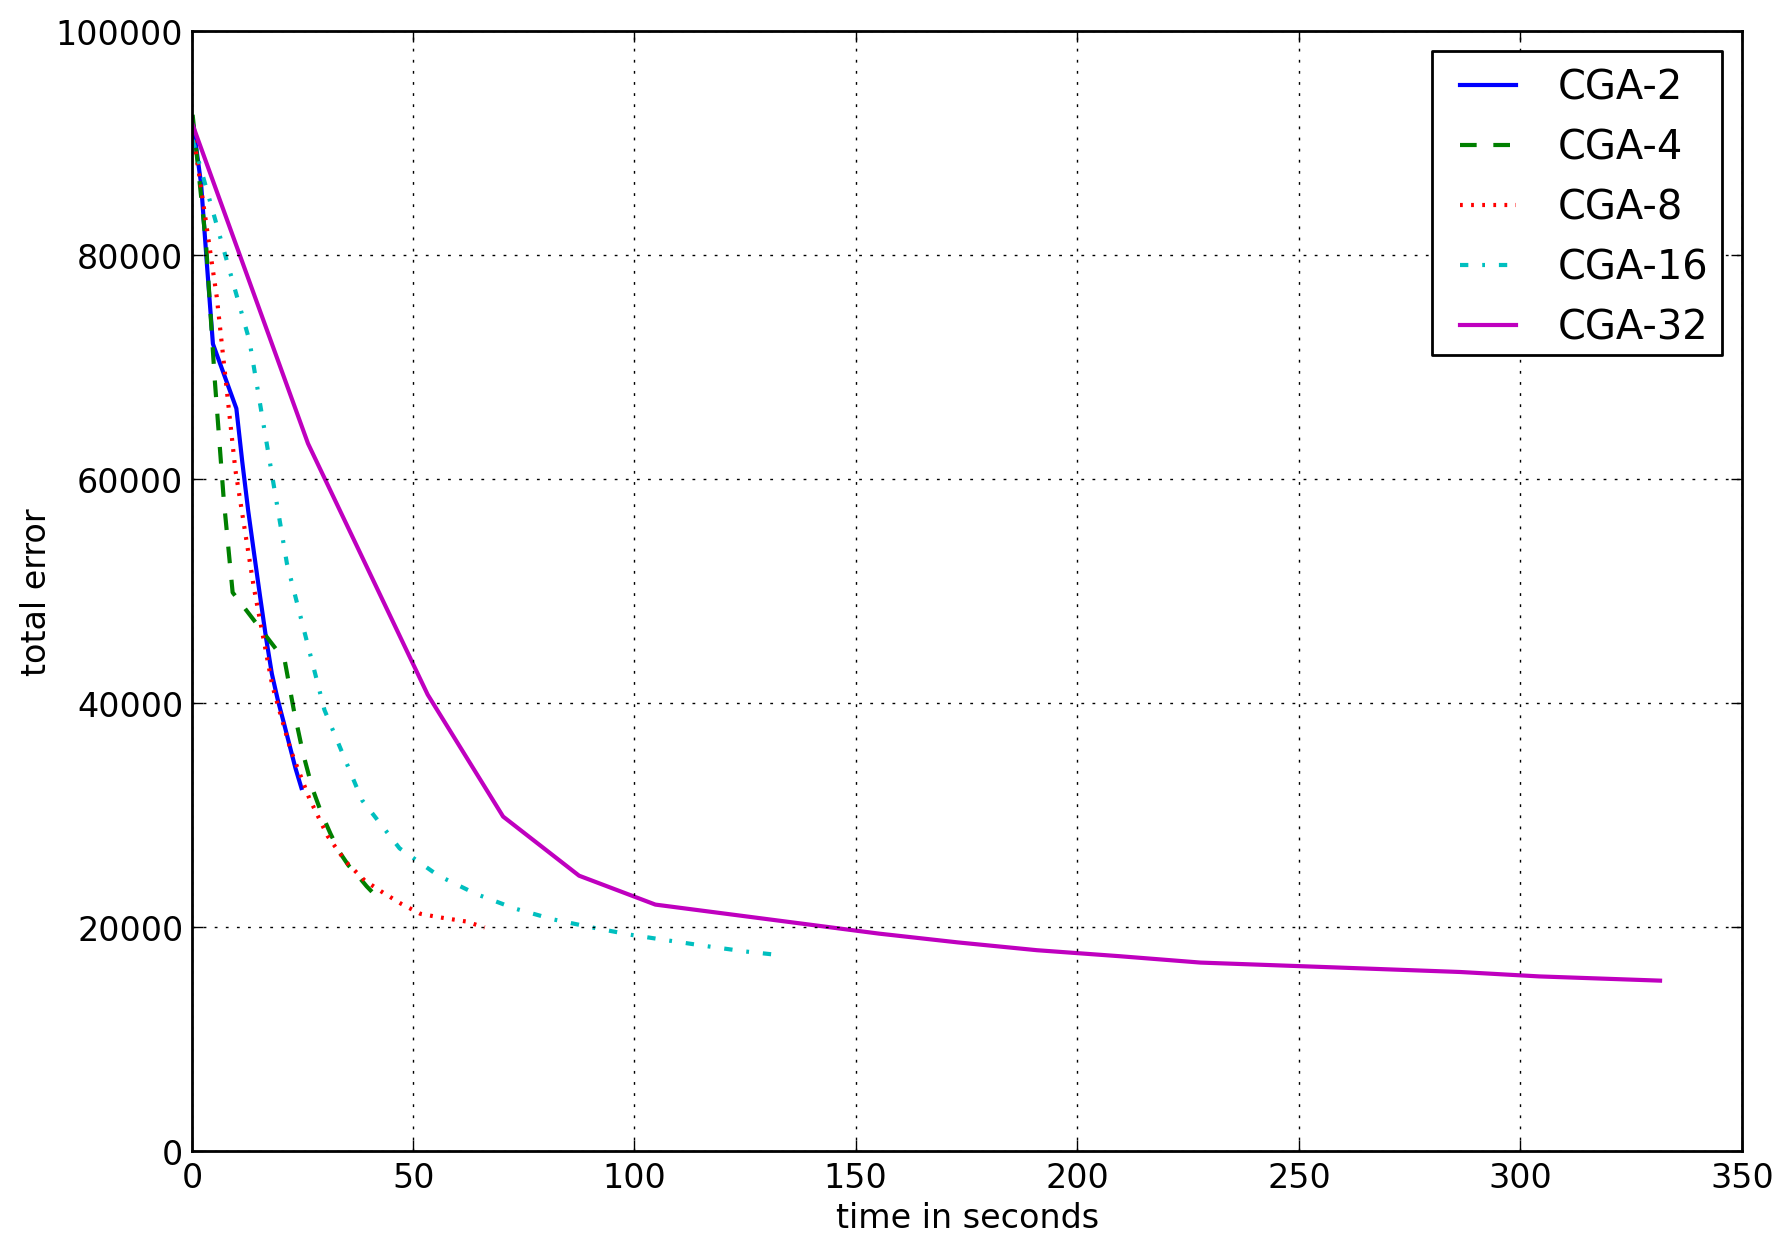
\includegraphics[width=0.45\linewidth]{ga_comparison4_2.png}
  }
  \caption{Comparison of performance for CGA and HGA with population sizes of 2, 4, 8, 16, and 32. HGA performs significantly better than CGA in terms of final reconstruction error.}
  \label{fig:ga_comparison4}
\end{figure*}
